% !TEX program = pdflatex
\documentclass[aspectratio=169, 10pt]{beamer}

% Theme 
\usetheme{metropolis}
\metroset{
 titleformat=regular,
 sectionpage=progressbar,
 numbering=fraction,
 progressbar=frametitle
}

% Packages 
\usepackage[T1]{fontenc}
\usepackage{graphicx}
\usepackage{booktabs}
\usepackage{appendixnumberbeamer}

% Colors 
\definecolor{accent}{HTML}{2563EB}
\setbeamercolor{frametitle}{bg=accent, fg=white}
\setbeamercolor{progress bar}{fg=accent}
\setbeamercolor{title separator}{fg=accent}
\setbeamercolor{alerted text}{fg=accent}

% Graphic path 
\graphicspath{{../plots/}}

% Title metadata 
\title{Predicting Loan Default Risk}
\subtitle{Model Development \& Evaluation}
\author{Ranbir Brar}
\date{}
\titlegraphic{%
 \vfill
 \hfill
}

% ============================================================
\begin{document}
% ============================================================

% Title Page 
\begin{frame}[plain]
 \titlepage
\end{frame}

% ============================================================
% SECTION 1: Exploratory Data Analysis
% ============================================================
\section{Exploratory Data Analysis}

% Slide 1: Target Imbalance & Data Scope 
\begin{frame}{Target Imbalance \& Data Scope}
 \begin{columns}[T]

 \begin{column}{0.42\textwidth}
 \begin{itemize}
 \item Severe class imbalance in known outcomes
 (\textasciitilde85\% Repaid, \textasciitilde15\% Defaulted) standard
 accuracy is misleading; F1 and AUC are the right metrics.
 \vspace{0.5em}
 \item \textasciitilde8\% of applications are \texttt{ongoing} no
 ground-truth label available, excluded from training.
 \vspace{0.5em}
 \item Statistical tests confirm ongoing apps are
 distributed randomly; exclusion introduces
 minimal selection bias.
 \end{itemize}
 \end{column}

 \begin{column}{0.55\textwidth}
 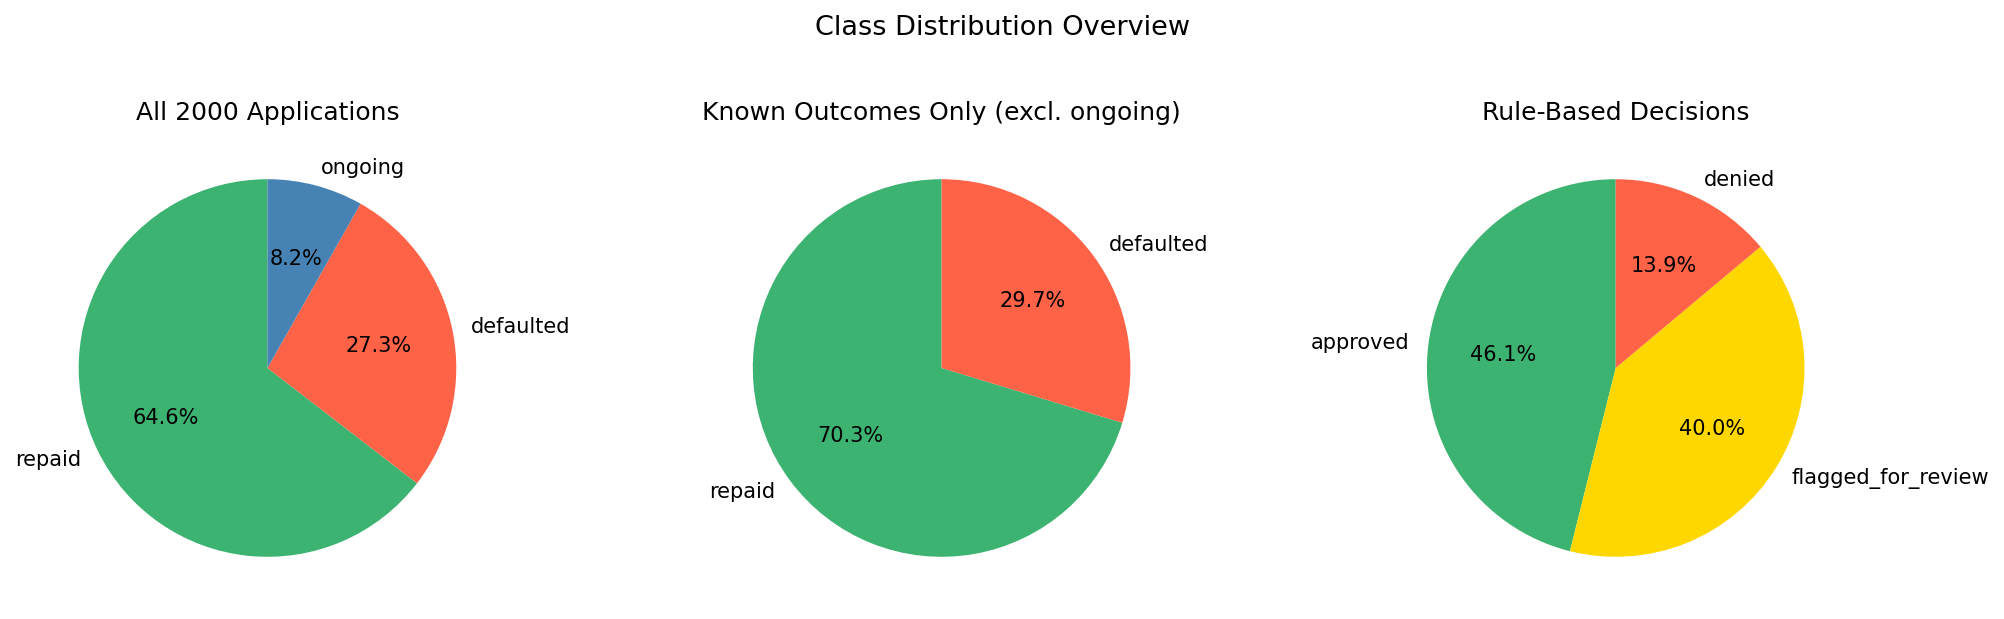
\includegraphics[width=\linewidth]{plot_02_class_distribution.png}
 \end{column}

 \end{columns}
\end{frame}

% Slide 2: Missing Data as a Predictive Signal 
\begin{frame}{Missing Data as a Predictive Signal}
 \begin{columns}[T]

 \begin{column}{0.42\textwidth}
 \begin{itemize}
 \item 15\% of applications are missing
 \texttt{documented\_monthly\_income}.
 \vspace{0.6em}
 \item Missingness is \alert{not random}; undocumented
 applicants default at a significantly higher rate.
 \vspace{0.6em}
 \item Missing documentation is a risk signal in its own
 right not merely a data quality issue.
 \end{itemize}
 \end{column}

 \begin{column}{0.55\textwidth}
 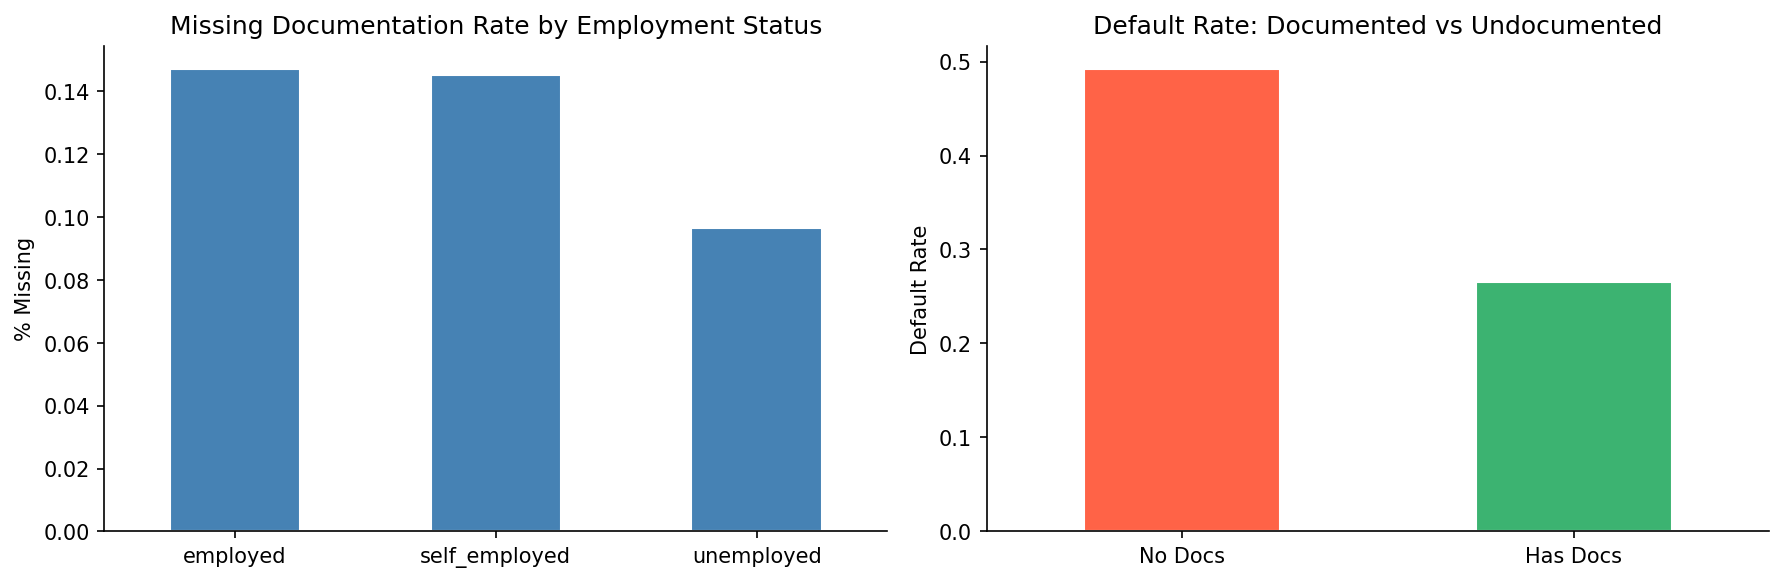
\includegraphics[width=\linewidth]{plot_01_missingness.png}
 \end{column}

 \end{columns}
\end{frame}

% Slide 3: Behavior Signals Over Raw Values 
\begin{frame}{Behaviour Signals Over Raw Values}
 \begin{columns}[T]

 \begin{column}{0.42\textwidth}
 \begin{itemize}
 \item When stated income is more than $2\times$
 documented income, default rates spike.
 Misrepresentation is a strong risk signal.
 \vspace{0.6em}
 \item Default rate jumps from \textasciitilde17\% to
 \textasciitilde42\% once the loan is more than
 30\% of monthly income.
 \vspace{0.6em}
 \item Raw dollar amounts matter less than how
 income \textit{relates} to the loan size.
 \end{itemize}
 \end{column}

 \begin{column}{0.55\textwidth}
 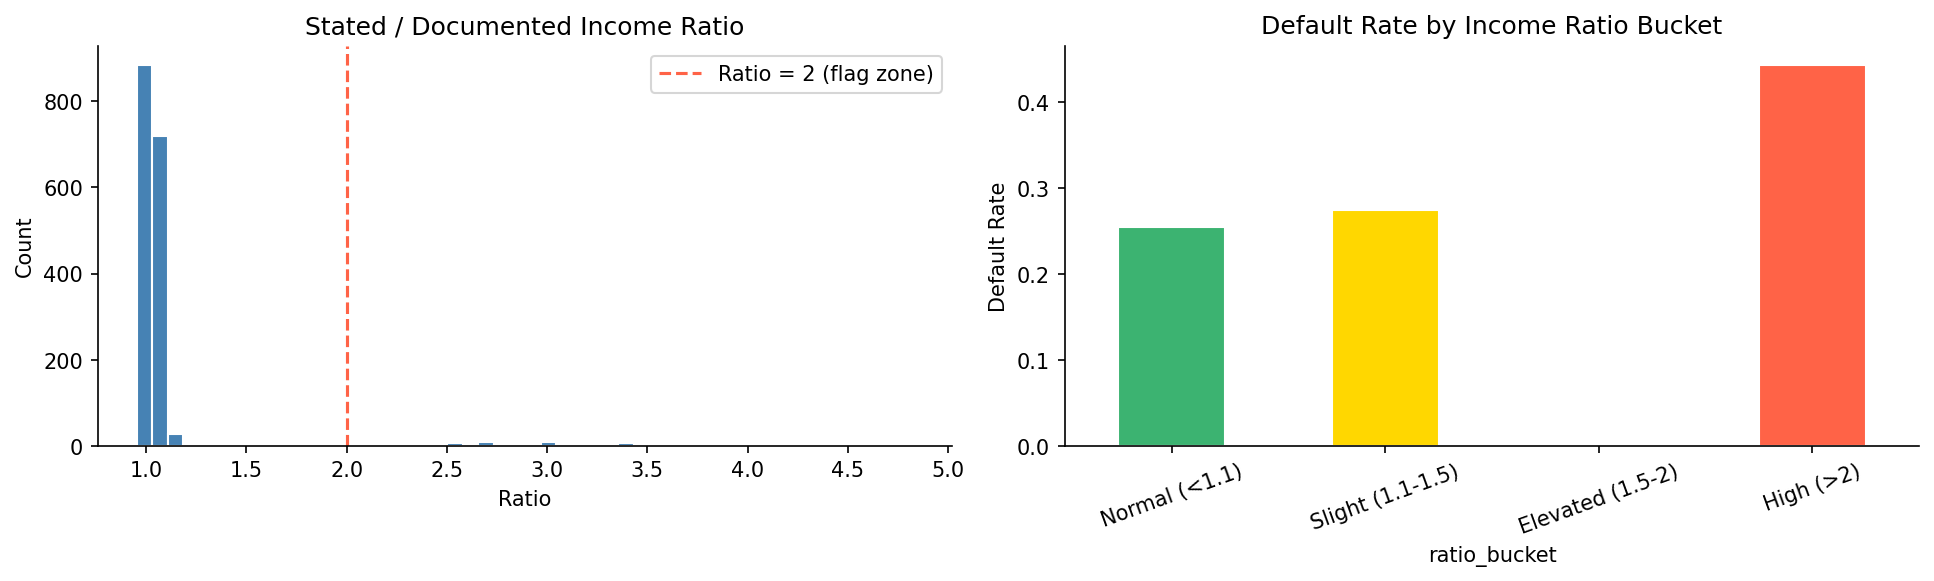
\includegraphics[width=\linewidth]{plot_03_income_misrepresentation.png}
 \end{column}

 \end{columns}
\end{frame}

% Slide 4: Loan-to-Income Stress Test 
\begin{frame}{Loan Size Relative to Income is the Key Signal}
 \begin{columns}[T]

 \begin{column}{0.42\textwidth}
 \begin{itemize}
 \item Default rate stays flat below 30\% LTI,
 then jumps sharply above it.
 \vspace{0.6em}
 \item Above 30\%, the applicant is likely
 stretched thin, even if their raw income
 looks fine.
 \vspace{0.6em}
 \item This is why \texttt{loan\_to\_income}
 becomes one of the strongest features
 in the model.
 \end{itemize}
 \end{column}

 \begin{column}{0.55\textwidth}
 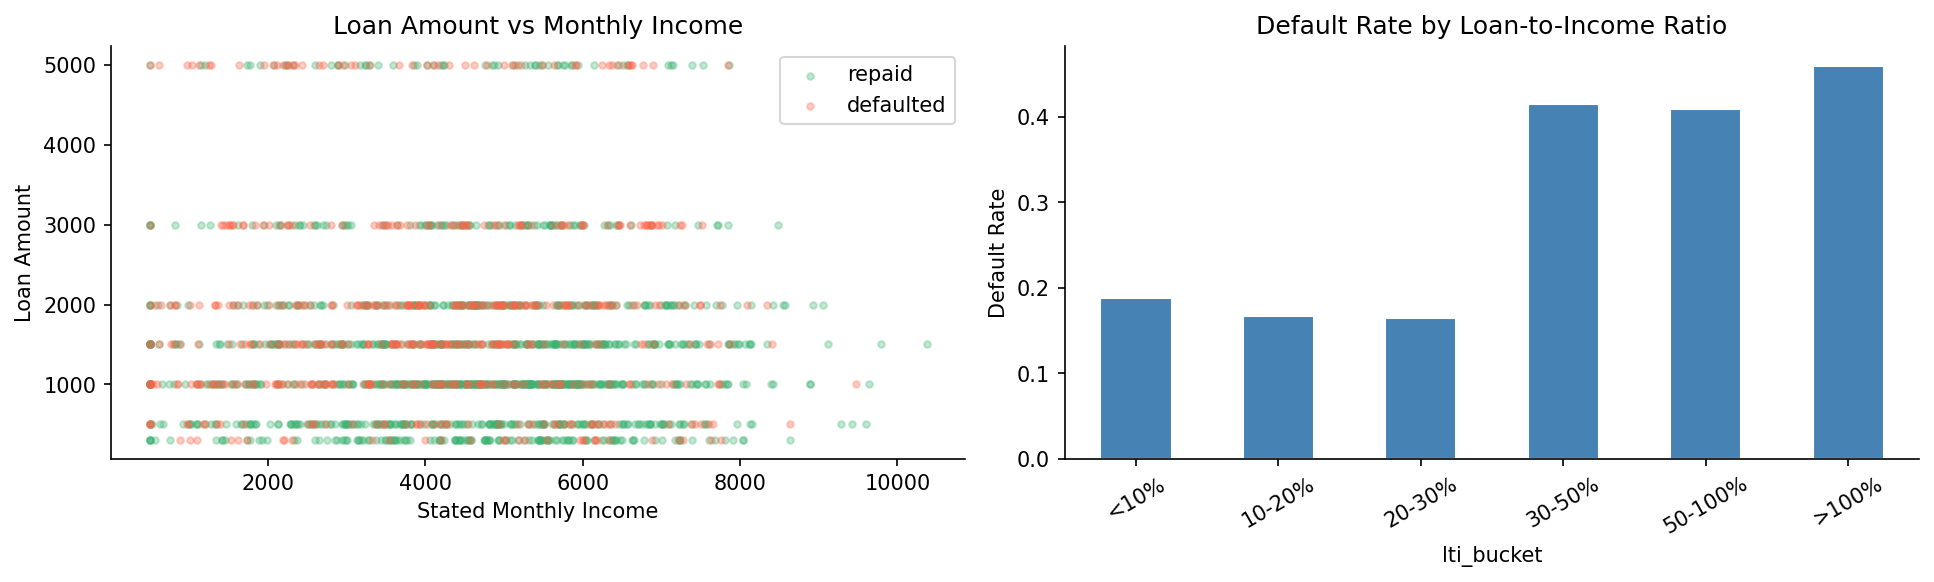
\includegraphics[width=\linewidth]{plot_07_loan_to_income.png}
 \end{column}

 \end{columns}
\end{frame}

% ============================================================
% SECTION 2: Model Choice
% ============================================================
\section{Model Choice}

% Slide 6: Why XGBoost? 
\begin{frame}{Why XGBoost?}
 \begin{columns}[T]

 \begin{column}{0.42\textwidth}
 \begin{itemize}
 \item Picks up non-linear interactions between
 features logistic regression can't do this.
 \vspace{0.5em}
 \item \texttt{scale\_pos\_weight} deals with class
 imbalance natively, no resampling needed.
 \vspace{0.5em}
 \item Threshold tuned for F1 on defaults,
 not the naive 0.5 cutoff.
 \end{itemize}

 \vspace{0.6em}
 \footnotesize
 \begin{tabular}{@{}ll@{}}
 \toprule
 5-fold CV AUC-ROC & $0.683 \pm 0.003$ \\
 Train size & 1{,}468 applicants \\
 Test size & 368 applicants \\
 \bottomrule
 \end{tabular}
 \end{column}

 \begin{column}{0.55\textwidth}
 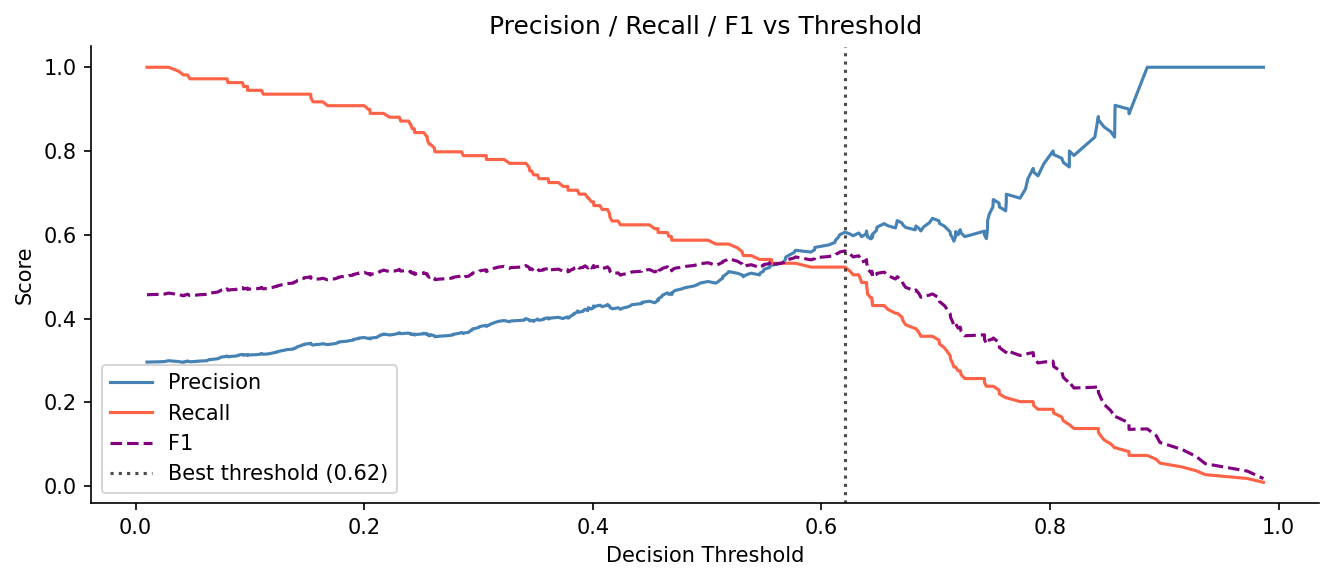
\includegraphics[width=\linewidth]{plot_threshold.png}
 \end{column}

 \end{columns}
\end{frame}

% Slide: Feature Correlations 
\begin{frame}{Why the Rule-Based Score Isn't Enough}
 \begin{columns}[T]

 \begin{column}{0.42\textwidth}
 \begin{itemize}
 \item Overdrafts and missing documentation
 are the strongest correlates with default.
 \vspace{0.6em}
 \item Bank balance and consistent deposits
 are negatively correlated, as expected.
 \vspace{0.6em}
 \item The rule-based score has weak correlation
 with actual outcomes. This is the gap
 the model is built to close.
 \end{itemize}
 \end{column}

 \begin{column}{0.55\textwidth}
 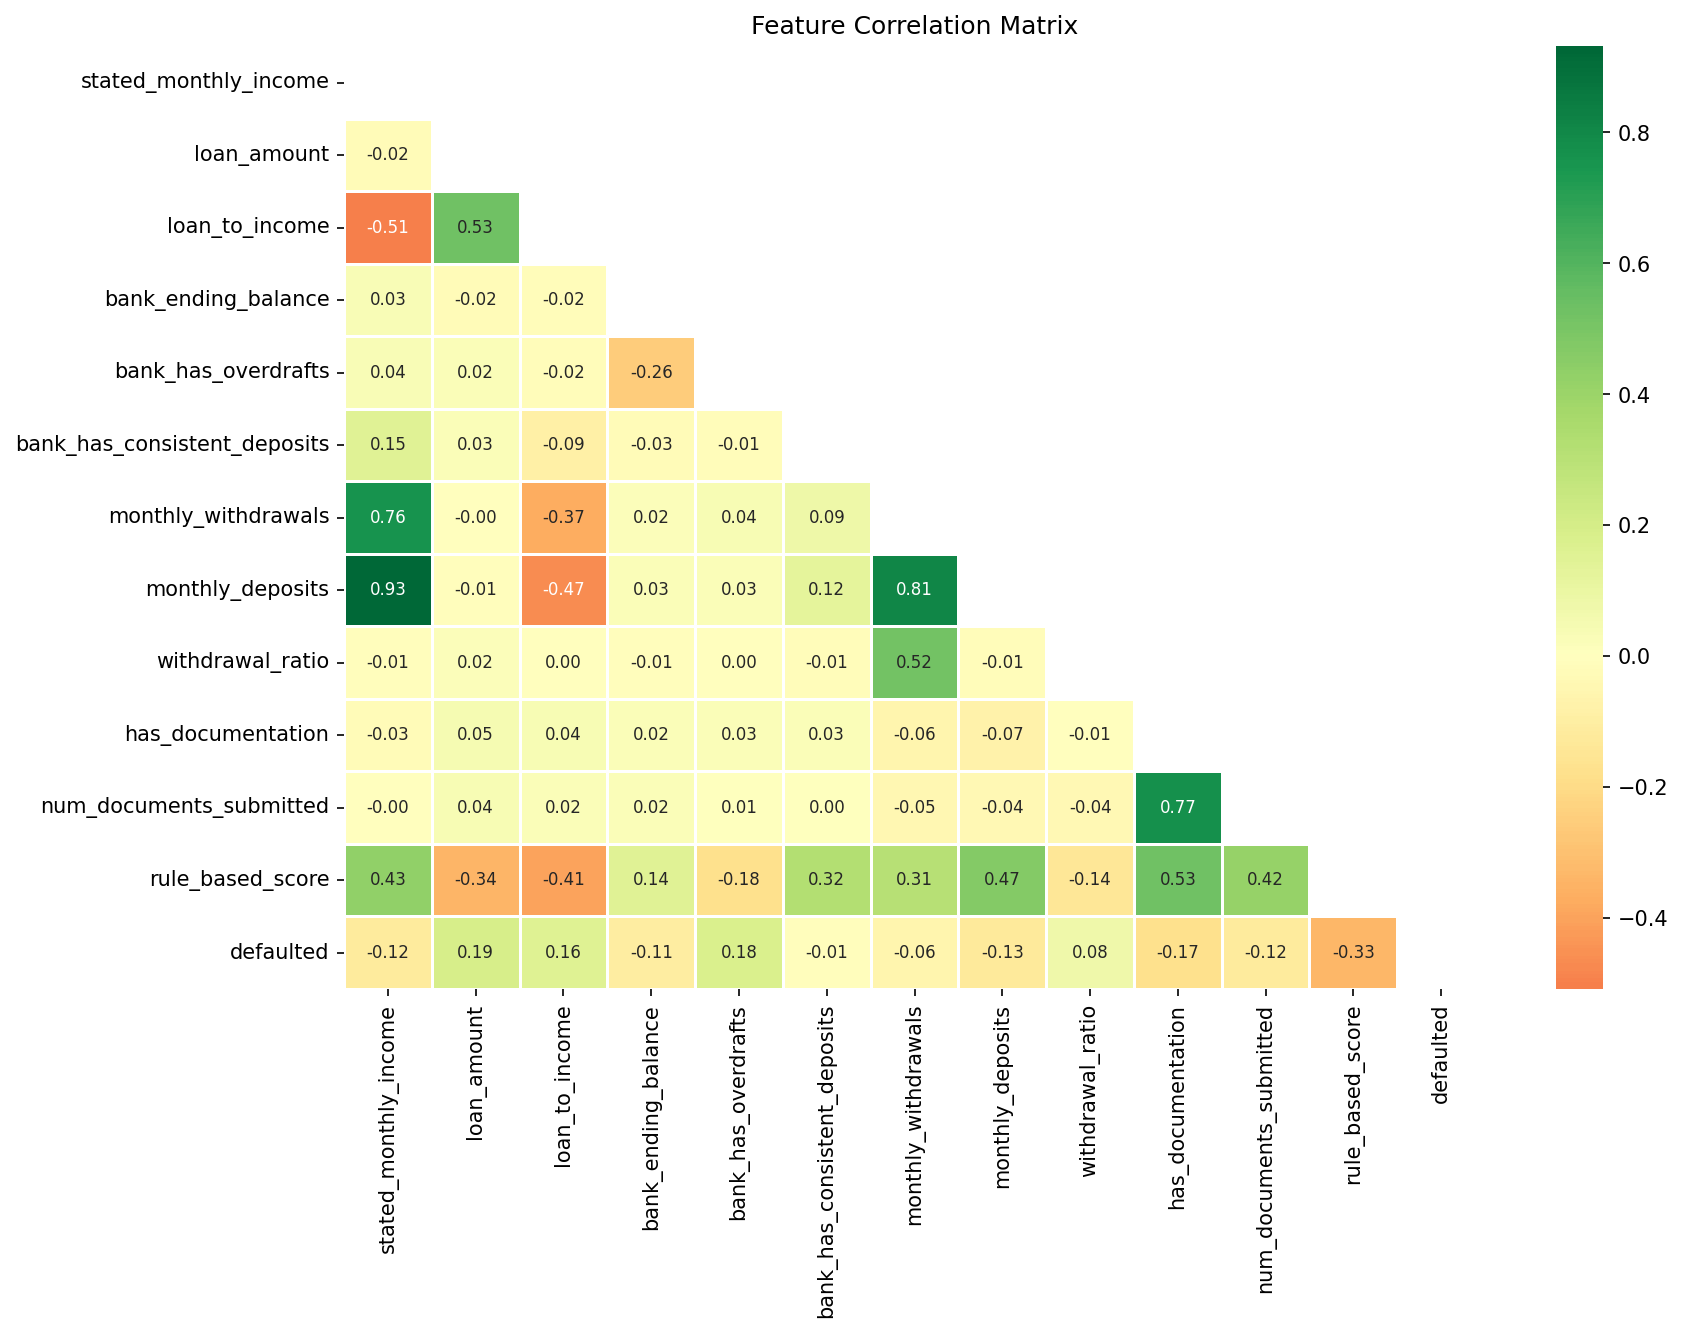
\includegraphics[width=\linewidth]{plot_06_correlations.png}
 \end{column}

 \end{columns}
\end{frame}

% Slide: What Drives Default Risk? 
\begin{frame}{What Drives Default Risk?}
 \begin{columns}[T]

 \begin{column}{0.42\textwidth}
 \begin{itemize}
 \item Gain-based importance pulled straight
 from the booster.
 \vspace{0.6em}
 \item \texttt{loan\_to\_income} and
 \texttt{withdrawal\_ratio} top the list 
 ratios beat raw numbers, same story as EDA.
 \vspace{0.6em}
 \item \texttt{has\_documentation} in top 5 
 not having docs is a red flag on its own.
 \end{itemize}
 \end{column}

 \begin{column}{0.55\textwidth}
 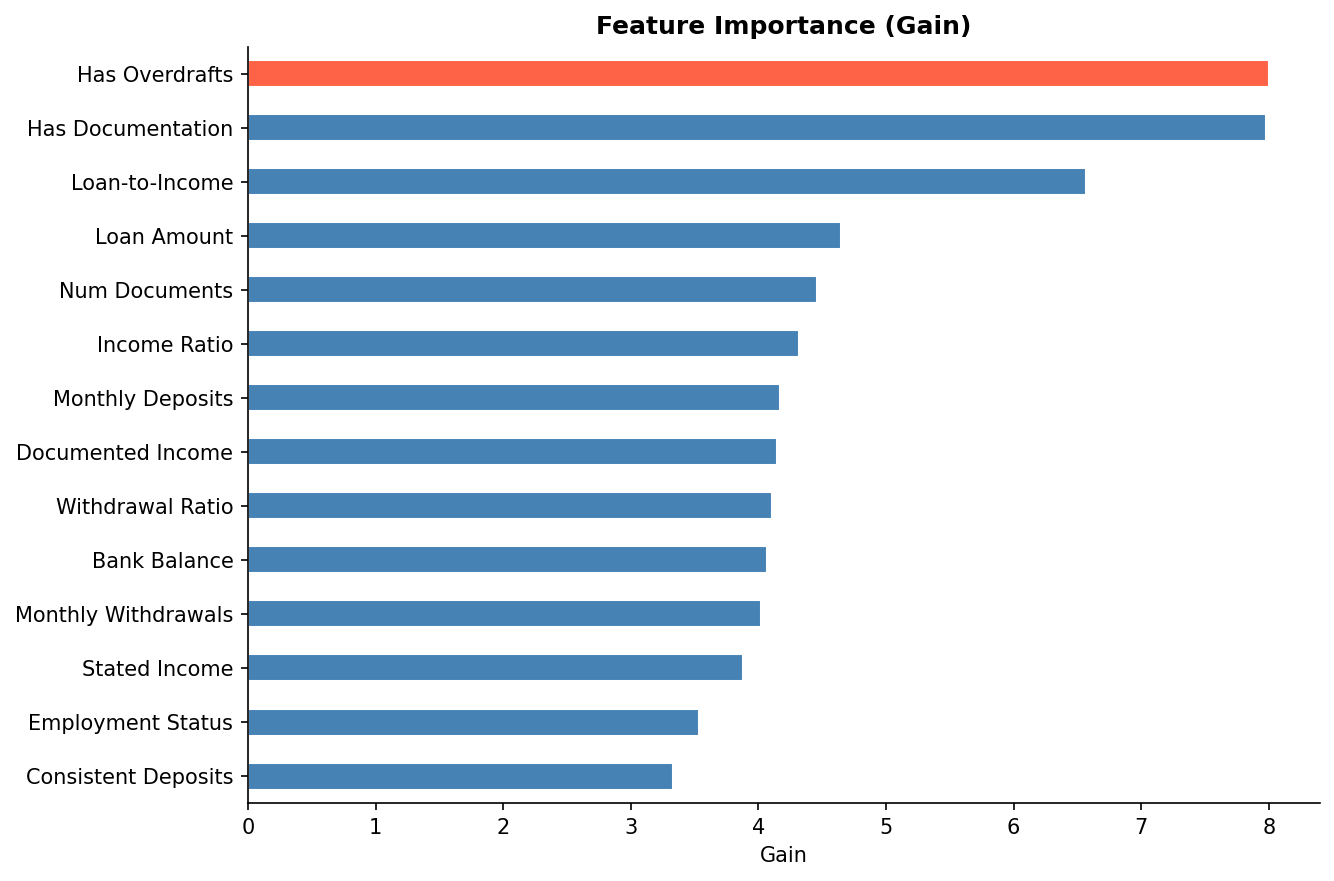
\includegraphics[width=\linewidth]{plot_shap_importance.png}
 \end{column}

 \end{columns}
\end{frame}

% Slide 6: Local Explainability 
\begin{frame}{Explaining Individual Decisions}
 \begin{columns}[T]

 \begin{column}{0.42\textwidth}
 \begin{itemize}
 \item Global importance $\neq$ why \alert{this}
 applicant got flagged.
 \vspace{0.6em}
 \item Each denial shows the top features and
 actual values for that person.
 \vspace{0.6em}
 \item Regulator asks why someone was denied?
 The explainer answers it automatically.
 \end{itemize}
 \end{column}

 \begin{column}{0.55\textwidth}
 \footnotesize
 \textbf{Applicant 1185} \hfill
 \alert{FLAG 80.3\% default probability}

 \vspace{0.5em}
 \begin{tabular}{@{}lcc@{}}
 \toprule
 Feature & Value & Gain \\
 \midrule
 Has Overdrafts & 0 & 8.0 \\
 Has Documentation & 0 & 8.0 \\
 Loan-to-Income & 1.133 & 6.6 \\
 Loan Amount & 2000 & 4.6 \\
 Num Documents & 0 & 4.5 \\
 \bottomrule
 \end{tabular}

 \vspace{0.5em}
 \scriptsize No documentation, no deposits, loan is
 $1.13\times$ monthly income. Each factor is
 visible and auditable.
 \end{column}

 \end{columns}
\end{frame}

% ============================================================
% SECTION 3: Evaluation
% ============================================================
\section{Evaluation}

% Slide 7: What the Metrics Actually Mean 
\begin{frame}{What the Metrics Actually Mean}
 \begin{columns}[T]

 \begin{column}{0.48\textwidth}
 \begin{itemize}
 \item \textbf{Precision:} of everyone flagged as a
 default, how many actually were? High precision
 means fewer good applicants wrongly denied.
 \vspace{0.5em}
 \item \textbf{Recall:} of all real defaults, how many
 did we catch? Low recall means defaults
 slipping through undetected.
 \vspace{0.5em}
 \item \textbf{F1:} balances precision and recall.
 More useful than accuracy when classes
 are imbalanced.
 \end{itemize}
 \end{column}

 \begin{column}{0.48\textwidth}
 \begin{itemize}
 \item \textbf{AUC-ROC:} ability to separate repayers
 from defaulters across all thresholds.
 0.5 is random, 1.0 is perfect.
 \vspace{0.5em}
 \item \textbf{FPR} (False Positive Rate): good
 applicants wrongly denied. A business cost.
 \vspace{0.5em}
 \item \textbf{FNR} (False Negative Rate): real defaults
 approved by mistake. A direct financial loss.
 \end{itemize}
 \end{column}

 \end{columns}
\end{frame}

% Slide 8: XGBoost vs. Rule-Based Baseline 
\begin{frame}{XGBoost vs.\ Rule-Based Baseline}
 \begin{columns}[T]

 \begin{column}{0.44\textwidth}
 \begin{table}
 \centering
 \footnotesize
 \begin{tabular}{@{}lccccc@{}}
 \toprule
 & Rec. & F1 & AUC & FPR & FNR \\
 \midrule
 XGBoost & 67.0\% & 53.5\% & 70.9\% & 35.1\% & 33.0\% \\
 Rule & 33.0\% & 43.1\% & 72.2\% & 8.5\% & 67.0\% \\
 \bottomrule
 \end{tabular}
 \end{table}

 \vspace{0.5em}
 \alert{FNR drops from 67\% to 33\%. XGBoost catches
 twice as many defaults as the rule-based system.}

 \vspace{0.4em}
 \footnotesize Rule-based looks more precise only
 because it flags almost nobody. Threshold of 0.62
 was tuned to maximise F1 on the default class.
 \end{column}

 \begin{column}{0.53\textwidth}
 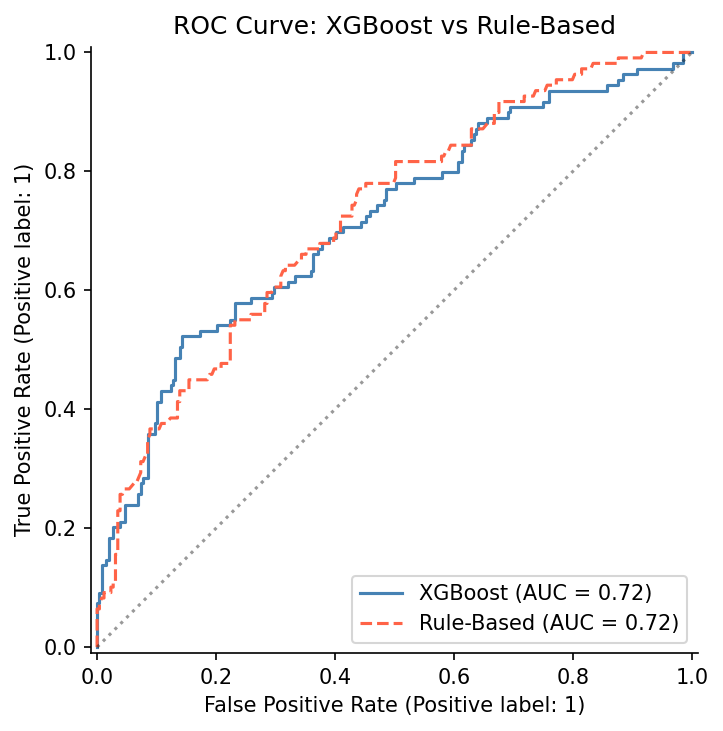
\includegraphics[width=\linewidth]{plot_roc_curves.png}
 \end{column}

 \end{columns}
\end{frame}

% Slide 9: The Deploy-Tomorrow Trade-off 
\begin{frame}{The Deploy-Tomorrow Trade-off}
 \begin{columns}[T]

 \begin{column}{0.42\textwidth}
 \begin{itemize}
 \item XGBoost catches \textbf{+37} more defaults per
 368 applications vs.\ baseline
 (recall goes from 33\% to 67\%).
 \vspace{0.5em}
 \item Cost: \textbf{+69} good applicants wrongly
 denied (FPR goes from 8.5\% to 35.1\%).
 \vspace{0.5em}
 \item \emph{Who decides?} The founders, weighing
 a missed default (full loan loss) against
 a lost customer (CAC). The threshold
 is a dial, not a fixed number.
 \end{itemize}
 \end{column}

 \begin{column}{0.55\textwidth}
 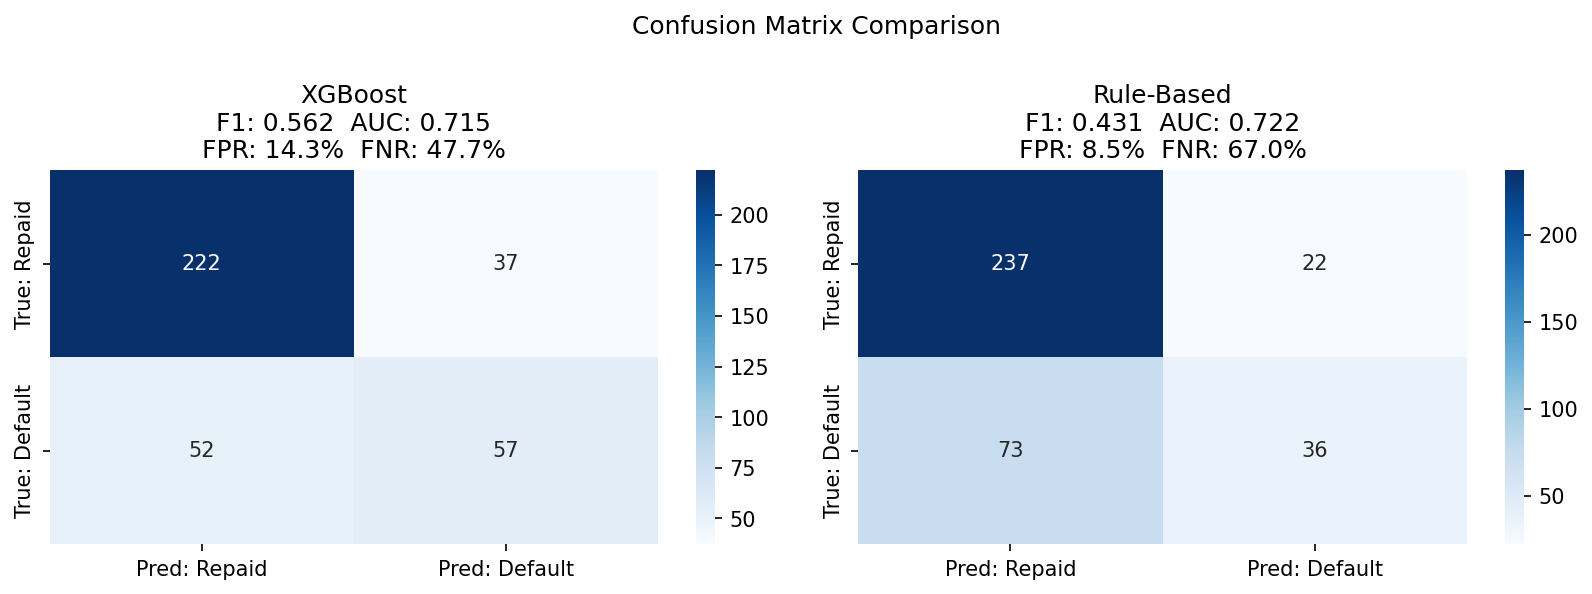
\includegraphics[width=\linewidth]{plot_confusion_matrices.png}
 \end{column}

 \end{columns}
\end{frame}

% ============================================================
% SECTION 4: Fairness & AI Ethics
% ============================================================
\section{Fairness \& AI Ethics}

% Slide: Fairness by the Numbers 
\begin{frame}{Where the Rule-Based System Fails on Fairness}
 \begin{columns}[T]

 \begin{column}{0.42\textwidth}
 \footnotesize
 \begin{tabular}{@{}lcccc@{}}
 \toprule
 Group & Default & Rule Appr. & ML Appr. \\
 \midrule
 Employed & 26.5\% & 56.3\% & 79.1\% \\
 Self-employed & 25.9\% & 34.8\% & 74.1\% \\
 Unemployed & 56.1\% & 0.0\% & 51.2\% \\
 \bottomrule
 \end{tabular}

 \vspace{0.6em}
 \normalsize
 \begin{itemize}
 \item Employed vs.~self-employed: nearly identical
 default rates, but the rule approves them
 at 56\% vs.~35\%. \alert{No risk justification
 for that 21-point gap.}
 \vspace{0.4em}
 \item XGBoost brings it to 79\% vs.~74\%,
 much closer to the actual risk split.
 \end{itemize}
 \end{column}

 \begin{column}{0.55\textwidth}
 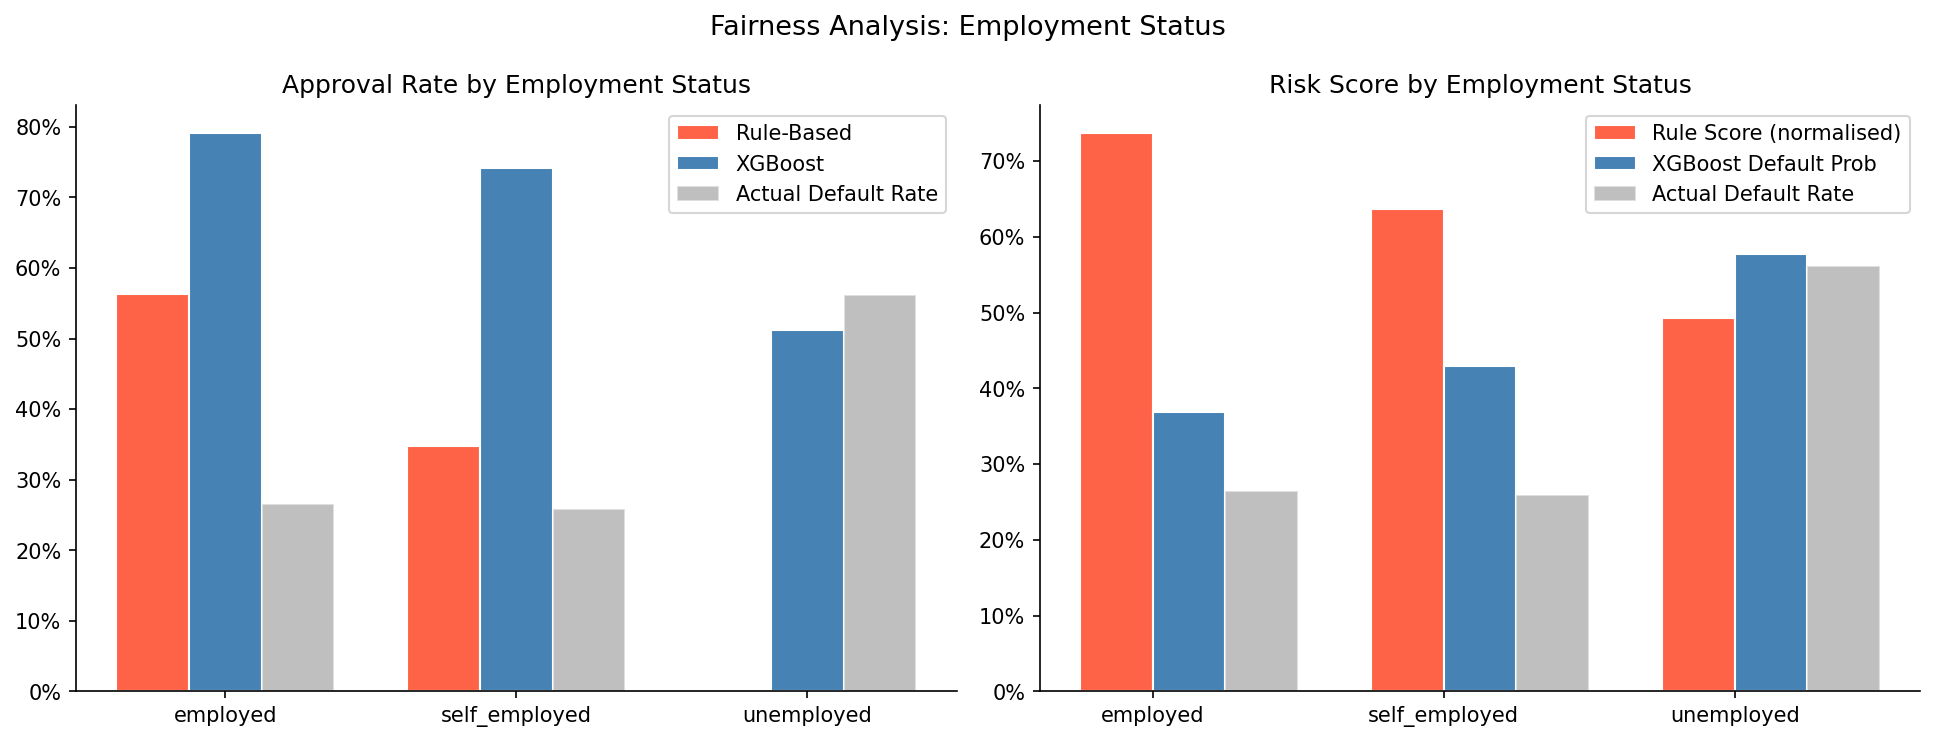
\includegraphics[width=\linewidth]{plot_fairness.png}
 \end{column}

 \end{columns}
\end{frame}

% Slide: AI Ethics 
\begin{frame}{The Harder Question: Should We Even Use This?}
 \begin{columns}[T]

 \begin{column}{0.48\textwidth}
 \textbf{The case for the model}
 \begin{itemize}
 \item Decisions are based on actual repayment
 behaviour, not assumptions about job type.
 \vspace{0.4em}
 \item Every denial is explainable with
 specific, per-applicant evidence.
 \vspace{0.4em}
 \item Catches twice as many defaults, which
 keeps the lender solvent and able to
 serve more customers.
 \end{itemize}
 \end{column}

 \begin{column}{0.48\textwidth}
 \textbf{The unresolved tensions}
 \begin{itemize}
 \item \texttt{employment\_status} is a proxy
 for protected characteristics. Even
 correct use carries disparate-impact risk.
 \vspace{0.4em}
 \item The model learned from historical loans.
 If past decisions were biased, it
 inherits that bias.
 \vspace{0.4em}
 \item An applicant denied by an algorithm
 has less recourse than one denied
 by a human. That matters.
 \end{itemize}
 \end{column}

 \end{columns}

 \vspace{0.5em}
 \footnotesize \emph{The right answer is not ``use the model'' or ``don't use it.''
 It is to deploy it with ongoing audits, a human review layer for edge cases,
 and a clear process for applicants to contest decisions.}
\end{frame}

% ============================================================
% SECTION 5: Production
% ============================================================
\section{Production}

% Slide 10: If This Went Live Tomorrow... 
\begin{frame}{If This Went Live Tomorrow\ldots}
 \begin{itemize}
 \item \textbf{Model drift:} a recession doubling default rates
 would silently degrade predictions unlike the rule-based
 system, which degrades \textit{transparently} and
 \textit{predictably}.
 \vspace{0.6em}
 \item \textbf{Distribution monitoring:} feature distributions
 (e.g., \texttt{loan\_to\_income} under inflation) must
 be tracked continuously; the static rule-based system
 requires no such infrastructure.
 \vspace{0.6em}
 \item \textbf{Regulatory audits:} handled the local explainer
 is deployed alongside the prediction API to generate
 automated, human-readable denial reasons per applicant.
 \end{itemize}
\end{frame}

% ============================================================
\end{document}
